\documentclass[conference]{IEEEtran}
% Uncomment only if a funding footnote is required:
% \IEEEoverridecommandlockouts

\usepackage{cite}
\usepackage{amsmath,amssymb,amsfonts}
\usepackage{graphicx}
\usepackage{textcomp}
\usepackage{xcolor}
\usepackage{booktabs}
\usepackage{url}

% The first path supports this repository; the other two support Overleaf when
% the three PNG files are uploaded either to figures/ or the project root.
\graphicspath{{../figures/png/}{figures/}{./}}

\def\BibTeX{{\rm B\kern-.05em{\sc i\kern-.025em b}\kern-.08em
    T\kern-.1667em\lower.7ex\hbox{E}\kern-.125emX}}

\begin{document}

\title{EnergyPlus-Trained Hourly Heating and Cooling Demand Surrogates for the Vienna Building Stock}

\author{
\IEEEauthorblockN{Philipp Thunshirn}
\IEEEauthorblockA{\textit{Department of Industrial Engineering}\\
\textit{University of Applied Sciences Technikum Wien}\\
Vienna, Austria\\
philipp.thunshirn@technikum-wien.at}
% Add further authors with \and and another IEEEauthorblockN/IEEEauthorblockA.
}

\maketitle

\begin{abstract}
This study develops an EnergyPlus-trained surrogate for hourly heating and
cooling demand of the Vienna building stock. The stock comprises 134.6 million
square metres of gross floor area and is represented by eight residential and
nonresidential cohorts covering four construction periods. Each cohort is
simulated as a reference archetype, and the resulting demand intensity is
scaled by its Citiwatts floor area. Separate histogram gradient-boosting
models combine demand-state classification with magnitude regression.
Validation on complete calendar weeks excluded from training gives
coefficients of determination of 0.959 for heating and 0.975 for cooling.
After floor-area-weighted aggregation, annual city demand differs from
EnergyPlus by 1.7 percent for heating and 0.8 percent for cooling. Peak demand
is underestimated by 6.7 percent and 10.1 percent, respectively. The complete
EnergyPlus demand path takes 67.1 seconds for the eight annual cohort
simulations, whereas surrogate inference for the same 70,080 cohort-hours
takes 1.73 seconds. The resulting speedup is approximately 39.
\end{abstract}

\begin{IEEEkeywords}
building energy simulation, building stock, cooling demand, EnergyPlus,
heating demand, surrogate model, Vienna
\end{IEEEkeywords}

\section{Introduction}

Hourly heating and cooling profiles are an important input to energy-system
models with high shares of renewable energy. Annual demand alone does not show
when heat pumps draw electricity, when heating coincides with a winter peak,
or when cooling increases the summer load. These questions require a building
model that responds to weather, solar and internal gains, occupancy schedules,
the thermal envelope, and the operation of heating and cooling systems. Simple
degree-day relations or fixed normalized profiles can reproduce an annual
total, but they do not represent these interactions explicitly.

EnergyPlus provides a considerably richer description of building demand
\cite{Crawley2001,EnergyPlus2026}. It solves the transient heat balance and accounts for heat
transfer through opaque surfaces and windows, ventilation and infiltration,
solar radiation, internal gains, thermal storage, and HVAC controls. Heating
and cooling loads therefore follow from the same physical balance instead of
being imposed as independent profiles. EnergyPlus is also a widely used and
extensively documented building-performance simulation program. Its accuracy
still depends on appropriate geometry, material properties, schedules, and
weather. Given suitable inputs, however, it provides a more defensible basis
for deriving hourly building loads than a profile assembled from annual
energy and outdoor temperature alone.

The detail that makes EnergyPlus useful also complicates its integration into
larger models. A city-scale application requires several representative
buildings, input files and schedules, repeated annual simulations, and the
extraction of results from EnergyPlus output files. Direct coupling becomes
particularly burdensome when building demand is evaluated repeatedly in a
scenario analysis or optimization model. The building simulation can then
become a computational and technical bottleneck even when one annual run is
not prohibitively slow.

A surrogate model offers a practical division of work. EnergyPlus is retained
offline as the detailed teacher, while a statistical model learns the mapping
from weather, operating conditions, and building properties to useful heating
and cooling demand. Once trained, the surrogate can be called directly by an
energy-system model without constructing and executing a new EnergyPlus run
\cite{Westermann2019,Amasyali2018}. The gain in speed is only useful if the surrogate preserves
annual energy, hourly variation, seasonal transitions, and peak demand.

This paper demonstrates the approach for the Vienna building stock. Citiwatts
floor area and construction-period data are represented by eight residential
and nonresidential cohorts. EnergyPlus simulations for the 2023 weather year
provide hourly useful heating and cooling for each cohort, and a
gradient-boosting surrogate emulates these outputs. The analysis assesses
hourly accuracy on periods excluded from training, accuracy after aggregation
to the Vienna stock, and computational performance. Building flexibility,
dispatch, and energy-system optimization are outside the present scope.

\section{Materials and Methods}

\subsection{Case Study and Building-Stock Representation}

The case study covers the Vienna building stock represented in the Citiwatts
inventory \cite{Citiwatts2026}. The inventory reports 134.6 million m\textsuperscript{2}
of gross floor area and 403.7 million m\textsuperscript{3} of heated volume.
Residential buildings account for 89.0 million m\textsuperscript{2}, and
nonresidential buildings account for 45.5 million m\textsuperscript{2}.
Reported annual heat consumption is 17.54 TWh. This quantity includes domestic
hot water and serves as a top-down energy-balance reference; it is distinct
from the useful space-heating output of the EnergyPlus simulations.

The stock was divided into residential and nonresidential buildings and four
construction periods: before 1975, 1975--1990, 1990--2000, and 2000--2014.
The corresponding raw shares were 54, 24, 4, and 17 percent and were normalized
before application within each sector. The resulting eight cohorts sum to the
complete Citiwatts floor area. They represent an aggregation of the Vienna
stock rather than a sample of individual buildings.

Table~\ref{tab:cohorts} reports the floor-area weights and principal thermal
parameters. Period-dependent U-values and residential geometry are informed
by Austrian TABULA and EPISCOPE apartment-building data
\cite{Loga2016,AustrianEnergyAgency2012}. The same
period-dependent U-value classes were used for nonresidential buildings
because an equivalent Vienna typology was unavailable. Residential window
solar transmittance values were derived from comparable TABULA window classes.
The nonresidential geometry, nonresidential solar transmittance, and areal heat
capacities are explicit model assumptions.

\begin{table*}[t]
\caption{Vienna Building-Stock Cohorts and Thermal Archetype Parameters}
\label{tab:cohorts}
\centering
\scriptsize
\setlength{\tabcolsep}{3.4pt}
\begin{tabular}{lrrrrrrrrr}
\toprule
Construction &
\multicolumn{2}{c}{Floor area (million m\textsuperscript{2})} &
\multicolumn{4}{c}{U-value (W/m\textsuperscript{2}K)} &
\multicolumn{2}{c}{Heat capacity (Wh/m\textsuperscript{2}K)} &
\multicolumn{1}{c}{$g_{\mathrm{res}}$} \\
\cmidrule(lr){2-3}\cmidrule(lr){4-7}\cmidrule(lr){8-9}
period & Residential & Nonresidential & Wall & Window & Roof & Floor &
Residential & Nonresidential & \\
\midrule
Before 1975 & 48.6 & 24.8 & 1.40 & 2.30 & 1.70 & 1.20 & 80 & 70 & 0.85 \\
1975--1990  & 21.6 & 11.0 & 1.10 & 2.70 & 0.80 & 0.80 & 75 & 65 & 0.76 \\
1990--2000  &  3.6 &  1.8 & 0.60 & 2.50 & 0.50 & 0.50 & 70 & 60 & 0.60 \\
2000--2014  & 15.3 &  7.8 & 0.35 & 1.40 & 0.20 & 0.40 & 65 & 55 & 0.50 \\
\midrule
Total & 89.0 & 45.5 & \multicolumn{7}{c}{} \\
\bottomrule
\multicolumn{10}{l}{\footnotesize Nonresidential window solar transmittance:
$g_{\mathrm{nonres}}=0.60$ for all periods.}
\end{tabular}
\end{table*}

Residential envelope-area ratios per unit conditioned floor area were 0.82
for walls, 0.18 for windows, 0.37 for roofs, and 0.36 for exposed floors.
The respective nonresidential ratios were 0.30, 0.12, 0.30, and 0.30.
Residential domestic-hot-water demand is separated in the wider Vienna data
set but is not simulated or predicted here. Citiwatts defines the stock extent
and supplies the floor-area weights for city aggregation. Its annual heat
consumption is not a surrogate target.

\subsection{EnergyPlus Reference Simulations}

One EnergyPlus 26.1 model was prepared for each cohort
\cite{EnergyPlus2026}. The models
represent equivalent stock archetypes rather than particular buildings. A
conditioned reference floor area of 1000 m\textsuperscript{2} was used in all
simulations. This common area keeps the geometry at a plausible archetype scale
and allows the output to be expressed as demand intensity. It does not restrict
the represented stock to 1000 m\textsuperscript{2}. Envelope areas, internal
gains, and air volumes were scaled consistently with the reference area.

The Citiwatts volume-to-area ratio gives a reference room height of
approximately 3 m and a conditioned volume of approximately 3000
m\textsuperscript{3}. Each archetype was simulated for the 8760 hours of 2023.
Outdoor temperature and solar radiation were obtained from Open-Meteo and
converted to a pseudo-EPW weather file \cite{Zippenfenig2023}. A
Climate.OneBuilding file
for Wien-Innere-Stadt supplied EPW header and format information, but not the
hourly observations \cite{ClimateOneBuilding2026}. Heating and cooling setpoints were 22 and
27~\textdegree C. The simulations included envelope transmission, solar and
internal gains, ventilation, infiltration, and ideal-load heating and cooling.

EnergyPlus outputs were converted to specific hourly demand
$q_{c,t}^{\mathrm{EP}}$ in kWh/m\textsuperscript{2}h. City-level demand was
obtained by multiplying the intensity by represented floor area $A_c$ and
summing across cohorts:
\begin{equation}
Q_{c,t}=q_{c,t}^{\mathrm{EP}}A_c,\qquad
Q_t^{\mathrm{Vienna}}=\sum_{c=1}^{8}Q_{c,t}.
\label{eq:aggregation}
\end{equation}
The procedure represents the complete inventory area through eight specific
demand profiles. It does not calibrate the EnergyPlus annual sum to the
17.54-TWh Citiwatts heat balance, which contains end uses outside the
EnergyPlus targets. The unnormalized EnergyPlus series is retained so that
teacher and surrogate are compared on the same basis.

\subsection{Dataset Generation and Preprocessing}

Combining eight cohort simulations with 8760 time steps produced 70,080
observations. One observation describes one cohort during one hour. The two
target variables are useful space-heating demand and useful cooling demand,
both in kWh/m\textsuperscript{2}h. Separate models were trained for the two
targets.

The explanatory variables comprise:
\begin{itemize}
\item weather: outdoor temperature and global horizontal, direct normal, and
diffuse horizontal irradiation;
\item operation: heating and cooling setpoints, internal gains, infiltration,
and ventilation air-change rates;
\item time: sine and cosine transformations of hour of day and day of year;
and
\item building properties: sector, cohort indicators, envelope U-values,
area ratios, and areal heat capacity.
\end{itemize}
The periodic time transformations avoid artificial discontinuities at midnight
and between calendar years. A specific heat-loss coefficient was calculated
from the products of U-values and their corresponding area ratios. Heating and
cooling temperature differences between outdoor temperature and the respective
setpoint, as well as their products with the heat-loss coefficient, were added
as physically meaningful predictors.

All cohort-hour combinations were retained; no random subsampling was applied.
Data preparation required eight complete annual profiles, checked for
duplicate cohort--timestamp pairs, and rejected missing values. Targets were
normalized by represented cohort area before fitting. Floor-area values were
used again only after prediction to obtain the city-level series.

\subsection{Surrogate Model}

Heating and cooling were modelled independently using the histogram-based
gradient-boosting implementation in scikit-learn
\cite{Friedman2001,scikit-learn,Ke2017}. Gradient
boosting constructs an additive ensemble of decision trees in which each
iteration reduces the residual error of the current ensemble. The model class
accommodates the mixture of continuous weather and envelope parameters, cyclic
time variables, and categorical cohort information.

Both targets contain long periods without demand. A single regression model
gave excessive influence to these hours and produced residual summer heating.
A two-part hurdle formulation was therefore used for each service. A
\texttt{HistGradientBoostingClassifier} first estimates the probability
$\widehat p_t$ that demand is present. A
\texttt{HistGradientBoostingRegressor} estimates demand magnitude
$\widehat q_t^{\mathrm{reg}}$. During inference,
\begin{equation}
\widehat q_t =
\begin{cases}
\max(0,\widehat q_t^{\mathrm{reg}}), & \widehat p_t \geq \tau,\\
0, & \widehat p_t < \tau,
\end{cases}
\label{eq:hurdle}
\end{equation}
where $\tau$ is a service-specific threshold.

Monotonic constraints were applied where the expected direction is
unambiguous. Predicted heating cannot increase with outdoor temperature and
increases with the heating temperature difference. Cooling follows the
opposite temperature response. The regression component used a learning rate
of 0.05, up to 700 boosting iterations, at most 159 leaf nodes per iteration,
and an L2 regularization coefficient of 0.01. The classifier used up to 300
iterations, 63 leaf nodes, and an L2 coefficient of 0.05.

\subsection{Training and Validation}

All 70,080 observations entered the cross-validation procedure. Sample weights
prevented moderate- and zero-demand hours from dominating the regression loss.
Positive observations up to the median positive demand received weight 2,
whereas the highest 15 percent of positive-demand observations received weight
9. Remaining observations received weight 1. Positive and zero classes were
balanced within each classifier training fold.

The hurdle threshold was selected independently in each training fold from
0.10 to 0.90 in increments of 0.05. Selection retained energy during true
on-hours while penalizing predictions during physically implausible off-hours.
Threshold selection used training-fold predictions only. The selected
threshold was 0.10 in all heating folds and ranged from 0.65 to 0.70 in the
cooling folds.

Temporal generalization was assessed by four-fold grouped cross-validation
using the ISO calendar week as grouping variable. All hours of a given week
and all eight cohorts were assigned to the same fold. Adjacent hours were
therefore not divided randomly between training and validation data. The
procedure evaluates unseen periods within 2023, but not a new building class
or an independent weather year.

Held-out cohort-hour predictions were evaluated with the coefficient of
determination, mean absolute error, and root mean squared error. Predictions
were then scaled according to \eqref{eq:aggregation}. Annual relative error,
peak-hour relative error, and Pearson correlation were calculated for the
fully out-of-fold Vienna series. Deployable models were finally refitted to
the complete data set; these fits were not used to report accuracy.

\subsection{Runtime Assessment}

The EnergyPlus runtime path included schedule and IDF generation, execution of
the simulation engine, and extraction of hourly results from the SQL output.
Engine time was measured three times per cohort and aggregated from the cohort
medians. Inference for both surrogate targets was repeated five times, and the
median duration was reported. Plot generation was disabled. The one-time
training duration was recorded separately and excluded from the inference
speedup.

\section{Results}

\subsection{EnergyPlus Cohort Response}

The EnergyPlus heat balances differ markedly between residential construction
periods, as shown in Fig.~\ref{fig:teacher}. During the selected winter day,
approximate transmission losses decline from about 82 W/m\textsuperscript{2}
for the pre-1975 cohort to about 26 W/m\textsuperscript{2} for the 2000--2014
cohort. Ventilation losses are similar because the same air-change assumption
is used across cohorts. Infiltration is omitted from the figure because its
common rate does not distinguish construction periods.

\begin{figure*}[t]
\centering
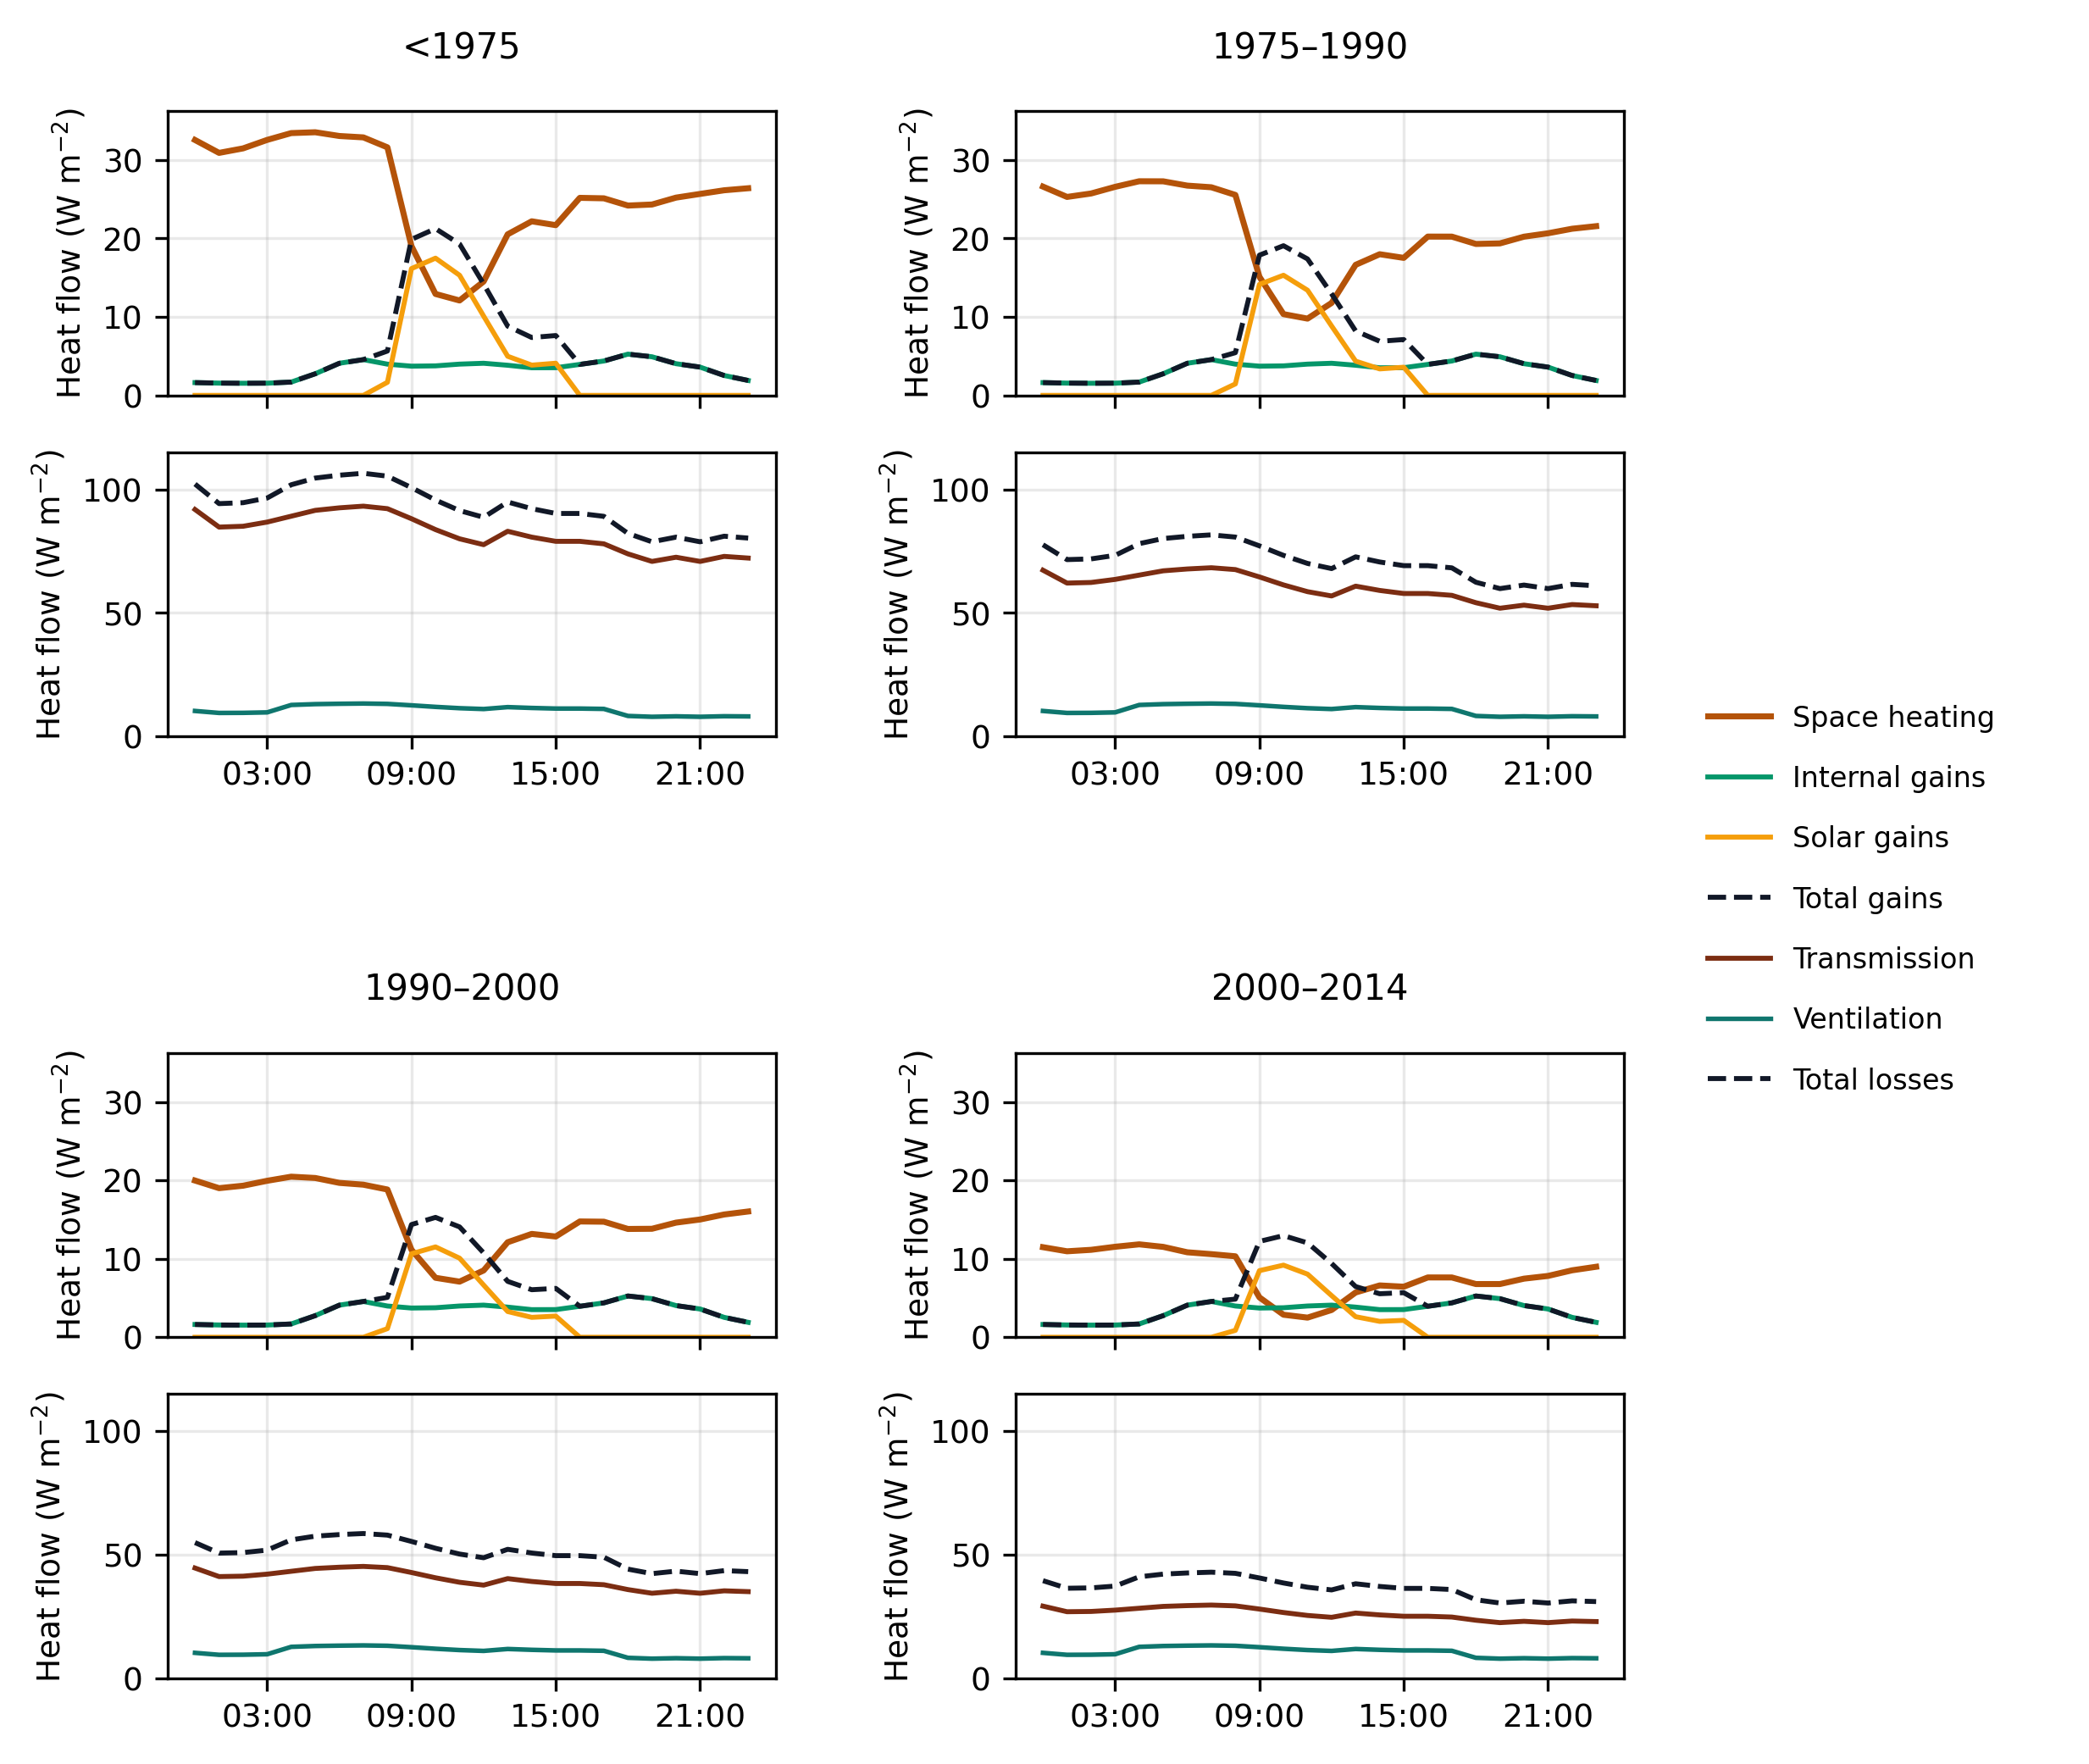
\includegraphics[width=\textwidth]{fig_01_teacher_flow_day.png}
\caption{EnergyPlus teacher heat-balance flows for four residential
construction periods during a winter day. Upper panels show space heating,
internal gains, solar gains, and total gains. Lower panels show approximate
transmission and ventilation losses.}
\label{fig:teacher}
\end{figure*}

\subsection{Surrogate Accuracy}

Table~\ref{tab:accuracy} summarizes out-of-fold accuracy. At cohort-hour level,
the surrogate reaches coefficients of determination of 0.959 for heating and
0.975 for cooling. After floor-area-weighted aggregation, annual city demand
differs from EnergyPlus by 1.7 percent for heating and minus 0.8 percent for
cooling. The temporal correlations are 0.982 and 0.989. Peak heating is
underestimated by 6.7 percent and peak cooling by 10.1 percent.

\begin{table}[t]
\caption{Calendar-Week Cross-Validation Results}
\label{tab:accuracy}
\centering
\footnotesize
\setlength{\tabcolsep}{3.5pt}
\begin{tabular}{lrr}
\toprule
Metric & Heating & Cooling \\
\midrule
Hourly $R^2$ & 0.959 & 0.975 \\
MAE (kWh/m\textsuperscript{2}h) &
$5.8{\times}10^{-4}$ & $5.4{\times}10^{-4}$ \\
City annual error (\%) & $+1.7$ & $-0.8$ \\
City peak-hour error (\%) & $-6.7$ & $-10.1$ \\
City Pearson $r$ & 0.982 & 0.989 \\
\bottomrule
\end{tabular}
\end{table}

Annual heating errors for the large residential cohorts remain within a few
percent. The largest cohort-relative error occurs for nonresidential buildings
from 2000--2014 at 23 percent. Their EnergyPlus heating intensity is only
3.8 kWh/m\textsuperscript{2}a; consequently, a small absolute deviation gives
a large percentage error and has little influence on the aggregate result.
Annual cooling errors remain within approximately 2 percent for all cohorts.

The seasonal weeks in Fig.~\ref{fig:weeks} show how aggregate errors are
distributed over time. During the peak-heating week, the surrogate follows the
daily variation but underestimates the highest loads; total weekly energy is
1.6 percent below EnergyPlus. In the early-April heating week, energy is
3.5 percent higher and the peak is closely reproduced. Cooling profiles in
late August and September agree closely in most hours, while the absolute
August peak remains underestimated.

\begin{figure*}[t]
\centering
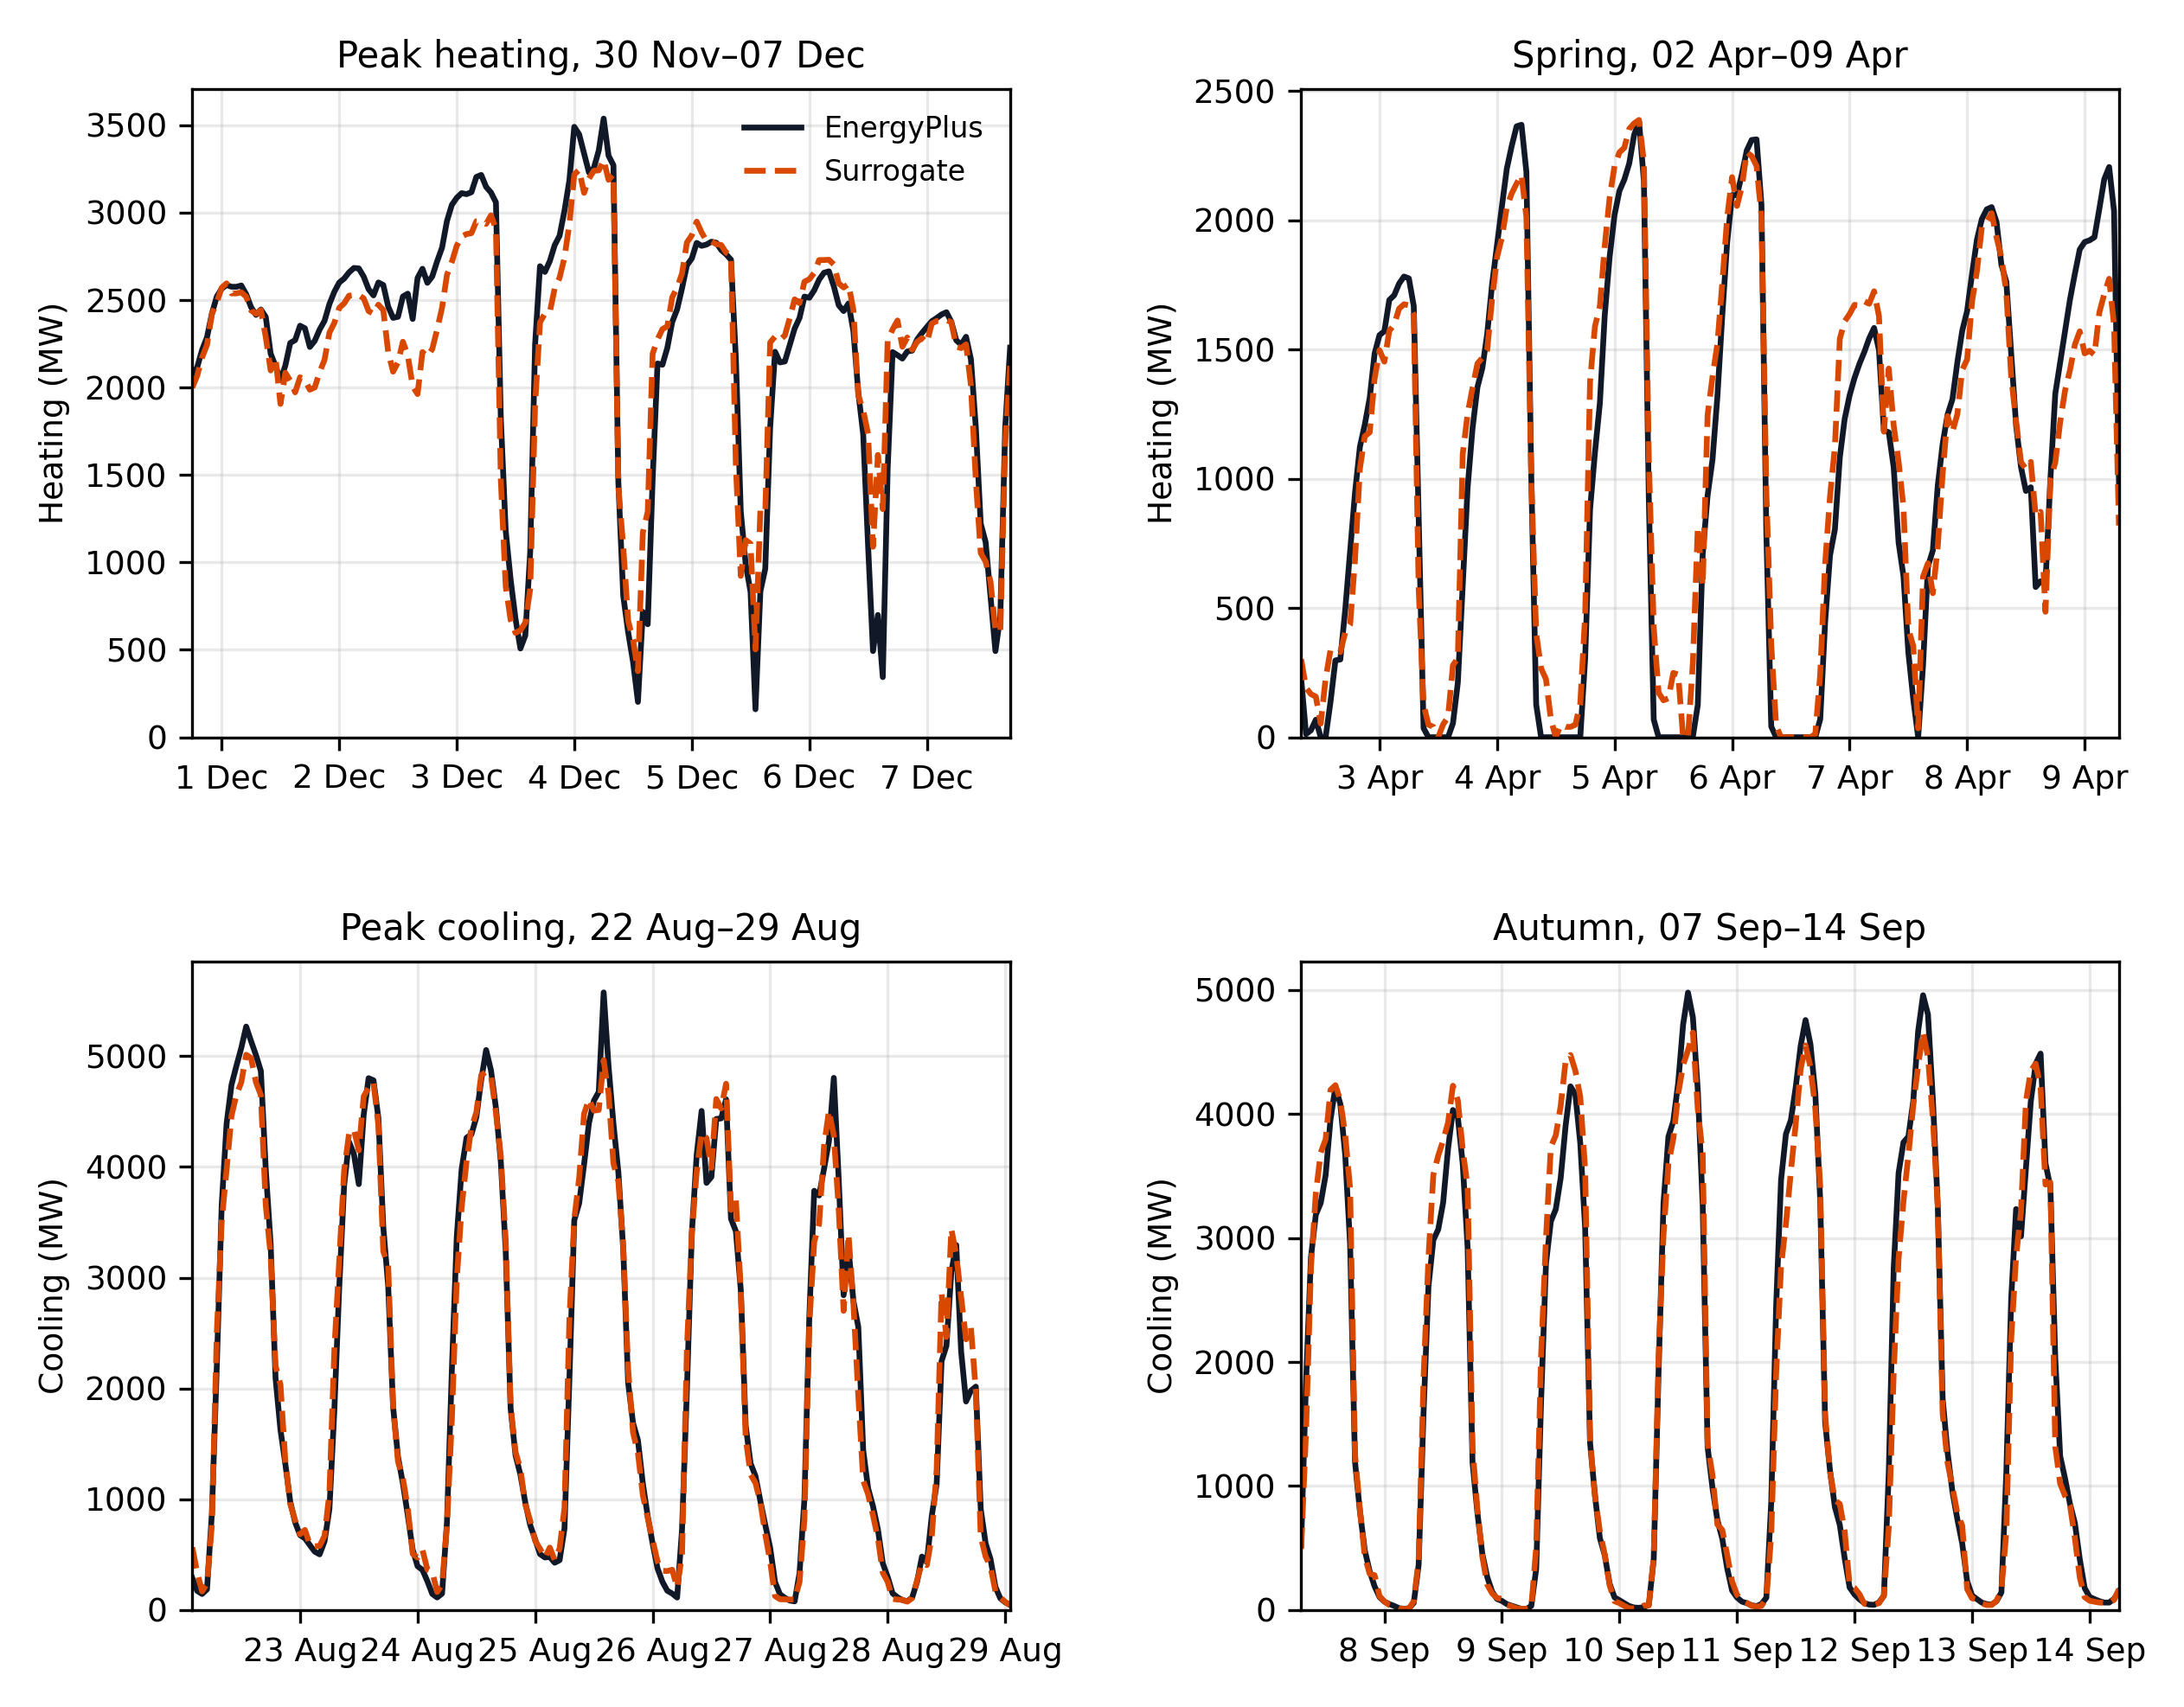
\includegraphics[width=0.96\textwidth]{fig_02_city_holdout_seasonal_weeks.png}
\caption{Floor-area-weighted Vienna useful demand from EnergyPlus and held-out
surrogate predictions. The panels show peak heating, April heating, peak
cooling, and September cooling. Each interval contains 168 consecutive hours.}
\label{fig:weeks}
\end{figure*}

Fig.~\ref{fig:temperature} relates city demand to outdoor temperature. The
1-K bin means produced by the surrogate follow those of EnergyPlus. Heating
decreases as outdoor temperature rises, whereas cooling increases at high
temperatures. The transition between both regimes is retained without a
substantial band in which both services are simultaneously overpredicted.

\begin{figure}[t]
\centering
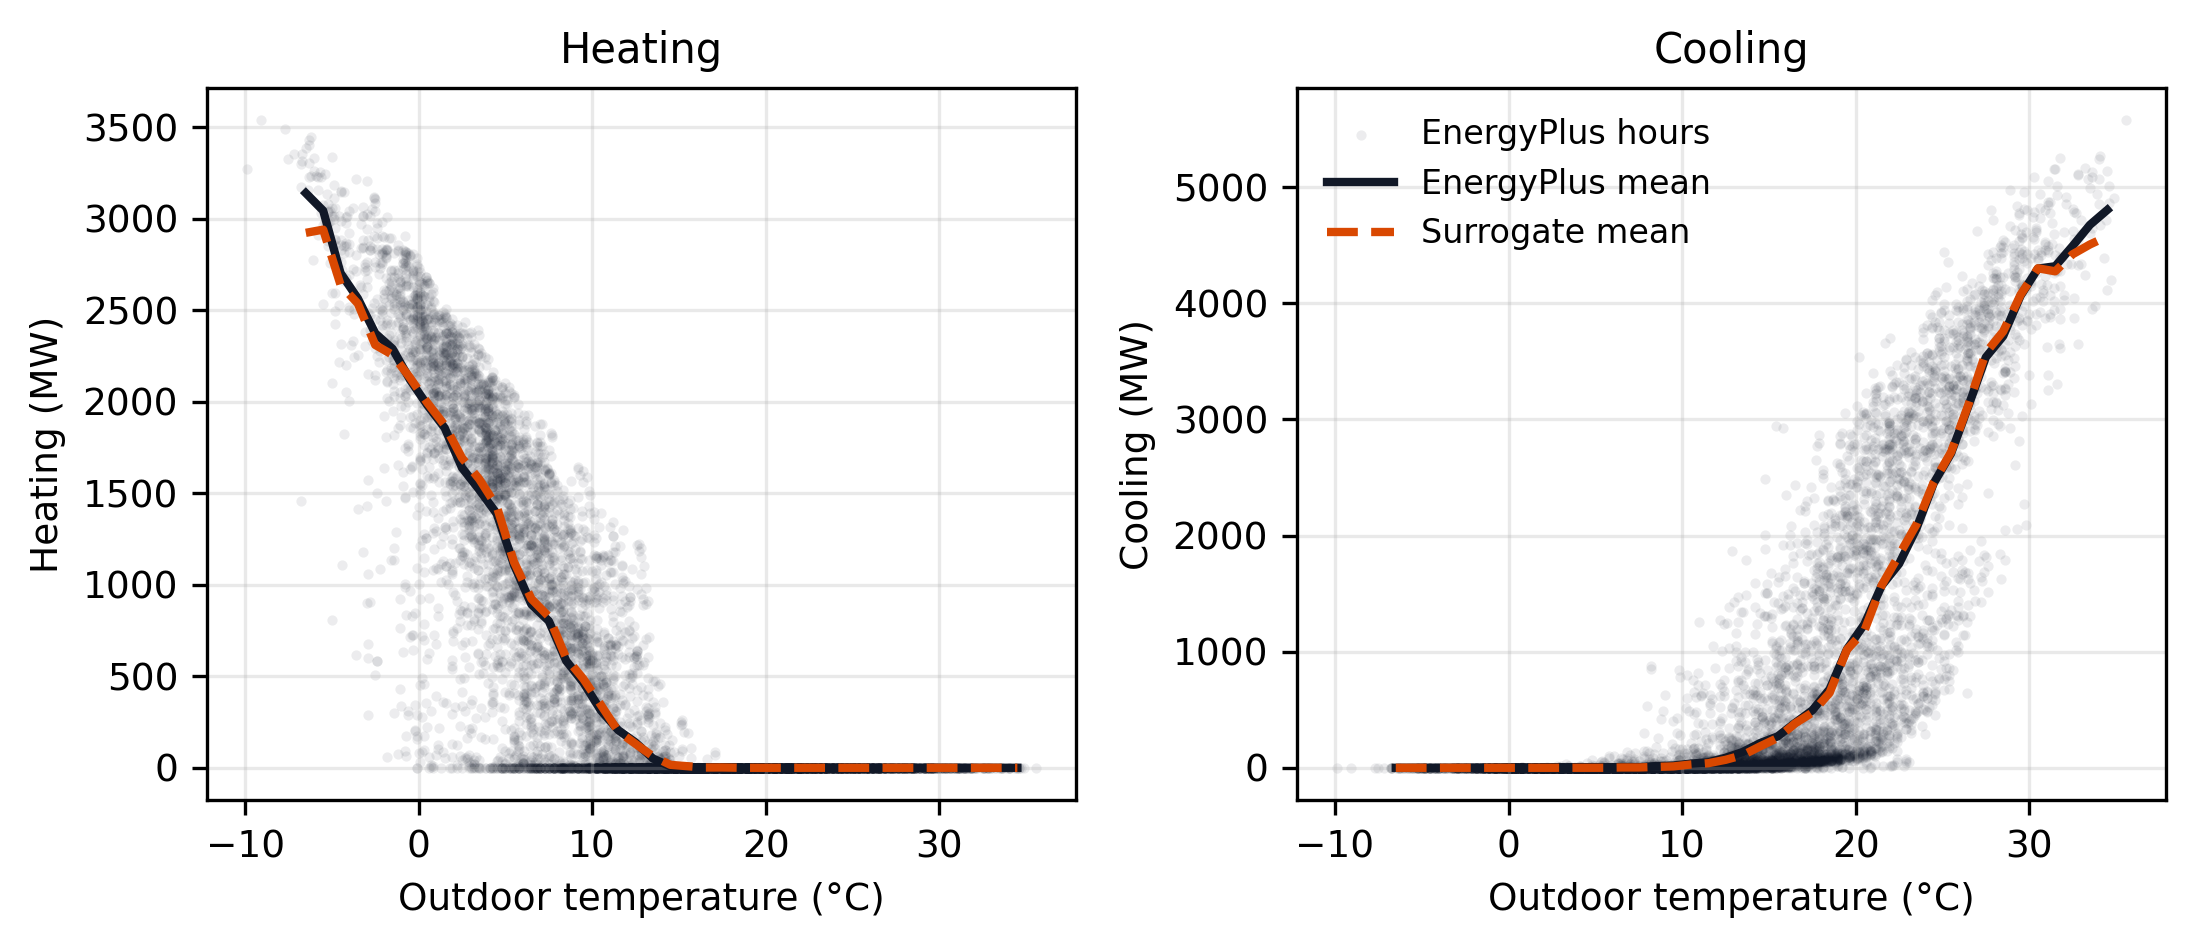
\includegraphics[width=\columnwidth]{fig_03_temperature_response.png}
\caption{Floor-area-weighted Vienna heating and cooling demand as a function
of outdoor temperature. Points show hourly EnergyPlus values. Lines show
EnergyPlus and surrogate means in 1-K temperature bins with at least eight
observations.}
\label{fig:temperature}
\end{figure}

EnergyPlus produces 0.43 GWh of heating from June through August, compared
with 1.84 GWh from the surrogate. This residual is small relative to the
approximately 5.3-TWh annual EnergyPlus space-heating series, but it shows
that the demand-state transition is not reproduced perfectly.

\subsection{Computational Performance}

The complete EnergyPlus demand path takes 67.1 s, including 27.5 s for input
preparation, 24.8 s for the simulation engine, and 14.8 s for SQL extraction,
as shown in Table~\ref{tab:runtime}. Surrogate inference for both targets takes
1.73 s, corresponding to a speedup of 38.8. Engine wall-clock time alone is
14.3 times the inference time. The one-time fit requires 18.5 s.

\begin{table}[t]
\caption{Runtime for Eight Cohorts and 8760 Hours}
\label{tab:runtime}
\centering
\footnotesize
\begin{tabular}{lrrrr}
\toprule
Path & Prep. & Engine & SQL & Total \\
 & (s) & (s) & (s) & (s) \\
\midrule
EnergyPlus & 27.5 & 24.8 & 14.8 & 67.1 \\
Surrogate inference & -- & -- & -- & 1.73 \\
\bottomrule
\end{tabular}
\end{table}

The inference comparison assumes that the hourly feature table is available;
its preparation is not included. For 50 repeated city-year evaluations, the
difference between both paths amounts to approximately 55 min.

\section{Discussion}

The results show that a compact statistical model can retain most of the
hourly variation generated by the EnergyPlus cohort simulations. Annual
energy and temporal correlation are reproduced more accurately than maximum
load. The surrogate is therefore suitable for producing hourly demand shapes
that are subsequently normalized to an independently specified annual energy
balance. It should not be used without qualification when the EnergyPlus
maximum itself is treated as a design load.

The city result covers all floor area in the Citiwatts inventory, but it does
not resolve every building in Vienna. Buildings within one sector and
construction period share an equivalent archetype and operating profile.
Aggregation retains major differences in envelope quality while suppressing
variation in geometry, occupancy, refurbishment, and control behaviour within
each cohort. Nonresidential archetypes carry additional uncertainty because
Vienna-specific geometry and window data were unavailable at the same level
as for Austrian residential apartment buildings.

Validation excludes complete calendar weeks from training, but remains limited
to one weather year and the same eight cohorts. The reported accuracy supports
interpolation across unseen periods of 2023, not transfer to a different
climate, an extreme year outside the training range, or an unseen building
type. The remaining peak-load underestimation is consistent with this
limitation.

The surrogate reproduces reference heating and cooling demand only. It does
not contain setpoint changes, preheating, load curtailment, rebound, or
indoor-temperature state transitions. These processes require a separate
stateful response model before building flexibility can be represented in an
optimization problem.

\section{Conclusion}

An EnergyPlus-to-surrogate workflow was developed for hourly useful heating
and cooling demand of the Vienna building stock. Eight archetypes represent
the complete Citiwatts floor area across two sectors and four construction
periods. Their EnergyPlus outputs form a 70,080-row annual data set. Separate
histogram gradient-boosting hurdle models reproduce held-out cohort-hour
demand with coefficients of determination of 0.959 for heating and 0.975 for
cooling.

After aggregation to the Vienna stock, annual errors remain below 2 percent,
whereas peak loads are underestimated by 7 to 10 percent. Surrogate inference
is approximately 39 times faster than the complete EnergyPlus demand path.
The model therefore provides an efficient source of EnergyPlus-consistent
demand profiles for subsequent energy-system analyses, provided that annual
energy anchors and peak-load limitations remain explicit.

\begin{thebibliography}{00}

\bibitem{Crawley2001}
D. B. Crawley, L. K. Lawrie, F. C. Winkelmann, W. F. Buhl, Y. J. Huang,
C. O. Pedersen, R. K. Strand, R. J. Liesen, D. E. Fisher, M. J. Witte, and
J. Glazer, ``EnergyPlus: Creating a new-generation building energy simulation
program,'' \textit{Energy and Buildings}, vol. 33, no. 4, pp. 319--331, 2001,
doi: 10.1016/S0378-7788(00)00114-6.

\bibitem{EnergyPlus2026}
U.S. Department of Energy, \textit{EnergyPlus Version 26.1.0 Documentation},
2026. [Online]. Available: \url{https://energyplus.net/documentation}.
Accessed: Aug. 28, 2026.

\bibitem{Westermann2019}
P. Westermann and R. Evins, ``Surrogate modelling for sustainable building
design---A review,'' \textit{Energy and Buildings}, vol. 198, pp. 170--186,
2019, doi: 10.1016/j.enbuild.2019.05.057.

\bibitem{Amasyali2018}
K. Amasyali and N. M. El-Gohary, ``A review of data-driven building energy
consumption prediction studies,'' \textit{Renewable and Sustainable Energy
Reviews}, vol. 81, pp. 1192--1205, 2018,
doi: 10.1016/j.rser.2017.04.095.

\bibitem{Citiwatts2026}
Citiwatts, ``Urban energy and building-stock indicators for Vienna,'' 2026.
[Online]. Available: \url{https://citiwatts.eu/}. Accessed: Aug. 28, 2026.

\bibitem{Loga2016}
T. Loga, B. Stein, and N. Diefenbach, ``TABULA building typologies in 20
European countries---Making energy-related features of residential building
stocks comparable,'' \textit{Energy and Buildings}, vol. 132, pp. 4--12,
2016, doi: 10.1016/j.enbuild.2016.06.094.

\bibitem{AustrianEnergyAgency2012}
Austrian Energy Agency, \textit{TABULA National Scientific Report Austria},
Vienna, Austria, 2012. [Online]. Available:
\url{https://episcope.eu/fileadmin/tabula/public/docs/scientific/AT_TABULA_ScientificReport_AEA.pdf}.
Accessed: Aug. 28, 2026.

\bibitem{Zippenfenig2023}
P. Zippenfenig, ``Open-Meteo.com Weather API,'' Zenodo, 2023,
doi: 10.5281/zenodo.7970649.

\bibitem{ClimateOneBuilding2026}
Climate.OneBuilding.Org, ``Repository of free climate data for building
performance simulation: Austria,'' 2026. [Online]. Available:
\url{https://climate.onebuilding.org/WMO_Region_6_Europe/AUT_Austria/index.html}.
Accessed: Aug. 28, 2026.

\bibitem{Friedman2001}
J. H. Friedman, ``Greedy function approximation: A gradient boosting
machine,'' \textit{The Annals of Statistics}, vol. 29, no. 5,
pp. 1189--1232, 2001, doi: 10.1214/aos/1013203451.

\bibitem{scikit-learn}
F. Pedregosa, G. Varoquaux, A. Gramfort, V. Michel, B. Thirion, O. Grisel,
M. Blondel, P. Prettenhofer, R. Weiss, V. Dubourg, J. Vanderplas, A. Passos,
D. Cournapeau, M. Brucher, M. Perrot, and E. Duchesnay, ``Scikit-learn:
Machine learning in Python,'' \textit{Journal of Machine Learning Research},
vol. 12, pp. 2825--2830, 2011.

\bibitem{Ke2017}
G. Ke, Q. Meng, T. Finley, T. Wang, W. Chen, W. Ma, Q. Ye, and T.-Y. Liu,
``LightGBM: A highly efficient gradient boosting decision tree,'' in
\textit{Advances in Neural Information Processing Systems}, vol. 30,
pp. 3146--3154, 2017.

\end{thebibliography}

\end{document}
